\section{SPARQL-DL}
\citet{evren_sirin} mengklasifikasikan bahasa query ontologi web semantik menjadi dua kelompok yaitu: bahasa query berbasis RDF \emph{(Resource Description Framework)} dan bahasa query berbasis DL \emph{(Description Logic)}. Bahasa query berbasis RDF ditujukan untuk melakukan query terhadap \emph{RDF Graph}. Bahasa query berbasis RDF diantaranya adalah SPARQL, SeRQL\footnote{http://rdf4j.org/} dan RDQL\footnote{http://www.w3.org/Submission/RDQL/}.

Ekspresi \emph{statement} bahasa query berbasis RDF seperti SPARQL, SeRQL dan RDQL berbasis pada bentuk \emph{RDF Triple} sehingga memiliki keterbatasan dalam melakukan query terhadap ontologi berbasis OWL 2 terutama OWL-DL. Misalnya terdapat ekspresi kelas dalam ontologi seperti ditunjukkan pada Persamaan \ref{eq:ekspresi_owldl} yang menyatakan bahwa terdapat sebuah kelas ``Dosen'' dengan kualifikasi anggota berupa individual dari kelas ``Orang'' yang memiliki relasi ``mengajar'' dengan individual kelas ``Mata\_Kuliah''. Apabila terdapat \emph{statement} seperti yang ditunjukkan pada Gambar \ref{fig:owl_entailment} maka SPARQL tidak dapat menemukan individual ``syamsul'' sebagai \emph{instance} kelas ``Dosen''.

\vspace{0.08cm}
\begin{equation}
	\label{eq:ekspresi_owldl}
	Dosen \equiv Orang \cap \exists mengajar.Mata\_kuliah 
\end{equation}
\vspace{0.08cm}

\begin{figure}[ht]
	\begin{lstlisting}[language=XML]
<ClassAssertion>
	<Class IRI="#Orang"/>
	<NamedIndividual IRI="#syamsul"/>
</ClassAssertion>
<ClassAssertion>
	<Class IRI="#Mata_Kuliah"/>
	<NamedIndividual IRI="#semantic_web"/>
</ClassAssertion>
<ObjectPropertyAssertion>
	<ObjectProperty IRI="#mengajar"/>
	<NamedIndividual IRI="#semantic_web"/>
	<NamedIndividual IRI="#syamsul"/>
</ObjectPropertyAssertion>\end{lstlisting}
\caption{Contoh ekspresi kelas ``Dosen'' dan Individual ``syamsul'' \emph{instance} dari kelas ``Orang''}
\label{fig:owl_entailment}
\end{figure}

Bahasa query berbasis \emph{Tripe pattern} tidak dapat mengekstraksi informasi berbasis ekspresi kompleks yang dihasilkan dari penggabungan definisi \emph{TBox} (class) dengan \emph{ABox} (individual). Beberapa penelitian yang dikemukakan untuk menangani keterbatasan bahasa query berbasis RDF diantaranya adalah \citet{evren_sirin}, \citet{kubias} dan \cite{fikes}. 

Bahasa query yang dikemukanan \cite{fikes} terbatas hanya pada query terhadap ekspresi \emph{TBox} sedangkan query SAIQL yang dikemukakan oleh \citet{kubias}. Bahasa query SPARQL-DL yang dikemukakan oleh \cite{evren_sirin} dapat diimplementasikan dengan menggunakan OWL-API. 

Arsitektur SPARQL-DL bekerja di atas \emph{library} OWL-API seperti ditunjukkan pada Gambar \ref{fig:sparqldl_architecture}. Bentuk \emph{statement} query SPARQL-DL mirip dengan \emph{statement} query SPARQL, perbedaan hanya terletak pada bentuk definisi klausa. Gambar \ref{fig:sparqldl_query_1} menunjukkan bentuk query SPARQL pada Gambar \ref{fig:sparql_select_1} jika ditransformasikan ke dalam bentuk SPARQL-DL. Contoh lain bentuk query SPARQL-DL ditunjukkan pada Gambar \ref{fig:sparqldl_query_2}. Ekspresi query yang didukung oleh SPARQL-DL cukup lengkap seperti ditunjukkan pada Tabel \ref{tab:sparqldl_expression}.

\begin{figure}[hb]
	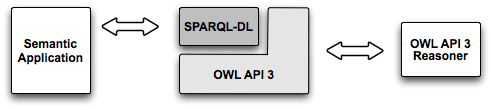
\includegraphics[width=1\textwidth]{bab_3/arsitektur_sparql_dl}
	\caption{Arsitektur SPARQL-DL}
	\label{fig:sparqldl_architecture}
\end{figure}

\begin{figure}[ht]
	\begin{lstlisting}[language=SQL, numbers=left]
PREFIX foaf: <http://xmlns.com/foaf/0.1/>
PREFIX : <http://danbri.org/foaf.rdf#>
select * where {
	PropertyValue(:danbri ?propery ?value)
}\end{lstlisting}
	\caption{Contoh query SPARQL-DL sederhana}
	\label{fig:sparqldl_query_1}
\end{figure}

\begin{figure}[ht]
	\begin{lstlisting}[language=SQL, numbers=left]
PREFIX wine: <http://w3.org/TR/2003/PR-owl-guide-20031209/wine#>
SELECT ?wine ?flavor WHERE { 
	PropertyValue(?wine, wine:locatedIn, wine:NewZealandRegion), 
	PropertyValue(?wine, wine:hasFlavor, ?flavor)
}\end{lstlisting}
	\caption{Contoh query SPARQL-DL dengan dua buah \emph{statement} kriteria}
	\label{fig:sparqldl_query_2}
\end{figure}

\begin{longtabu}{|c|l|X|}
	\caption{Daftar kelas ontologi geografi}\label{tab:sparqldl_expression}\\ \hline
	\textbf{No} & \textbf{Ekspresi Query}	&	\textbf{Keterangan}\\ \hline
	\endfirsthead
	\multicolumn{3}{c}%
	{\tablename\ \thetable\ {(lanjutan)}}\\ \hline
	\textbf{No} & \textbf{Ekspresi Query}	&	\textbf{Keterangan}\\ \hline
	\endhead
	1	&	Type(a,b)					&	\emph{a} adalah individual kelas \emph{b}\\ \hline
	2	&	Property(p)					&	\emph{p} adalah \emph{owl:Property}\\ \hline
	3	&	Class(a)					&	\emph{a} adalah \emph{owl:Class}\\ \hline
	4	&	Individual(a)				&	\emph{a} adalah \emph{owl:OWLNamedIndividual}\\	\hline
	5	&	PropertyValue(a, b, c)		&	\emph{a} memiliki properti \emph{b} dengan nilai \emph{c}\\ \hline
	6	&	EquivalentClass(a, b)		&	Kelas \emph{a} sama dengan \emph{b}\\ \hline
	7	&	SubClassOf(a, b)			&	\emph{a} sub kelas dari \emph{b}\\ \hline
	8	&	EquivalentProperty(a, b)	&	Properti \emph{a} sama dengan \emph{b}\\ \hline
	9	&	SubPropertyOf(a, b)			&	\emph{a} sub properti \emph{b}\\ \hline
	10	&	InverseOf(a, b)				&	Properti \emph{a} \emph{inverse} dari \emph{b}\\ \hline
	11	&	ObjectProperty(a)			&	\emph{a} adalah \emph{owl:ObjectProperty}\\ \hline
	12	&	DataProperty(a)				&	\emph{a} adalah \emph{owl:DataProperty}\\ \hline
	13	&	Functional(a)				&	\emph{a} memiliki karakteristik \emph{owl:Functional}\\ \hline
	14	&	InverseFunctional(a)		&	\emph{a} memiliki karakteristik \emph{owl:inverseFunctional}\\ \hline
	15	&	Transitive(a)				&	\emph{a} memiliki karakteristik \emph{owl:transitiveProperty}\\ \hline
	16	&	Symmetric(a)				&	\emph{a} memiliki karakteristik \emph{owl:symmetricProperty}\\ \hline
	17	&	Reflexive(a)				&	\emph{a} memiliki karakteristik \emph{owl:reflexive}\\ \hline
	18	&	Irreflexive(a)				&	\emph{a} memiliki karakteristik \emph{owl:irreflexive}\\ \hline
	19	&	SameAs(a, b)				&	\emph{a} memiliki karakteristik \emph{owl:sameAs}\\ \hline
	20	&	DisjointWith(a, b)			&	\emph{a} disjoint dengan \emph{b}\\ \hline
	21	&	DifferentFrom(a, b)			&	\emph{a} adalah individual yang berbeda dengan \emph{b}\\ \hline
	22	&	ComplementOf(a, b)			&	\emph{a} komplemen dari \emph{b}\\ \hline
	23	&	Annotation(a, b, c)			&	\emph{a} memiliki properti anotasi \emph{b} dengan nilai \emph{c} \emph{owl:Functional}\\ \hline
	24	&	StrictSubClassOf(a, b)		&	\emph{a} sub kelas (dengan aturan tertentu) dari \emph{b}\\ \hline
	25	&	DirectSubClassOf(a, b)		&	kelas \emph{a} berada langsung di bawah  \emph{b}\\ \hline
	26	&	DirectType(a, b)			&	individual \emph{a} merupakan \emph{instance} \emph{b} (sidpesifikan dalam \emph{statement})\\ \hline
	27	&	StrictSubPropertyOf(a, b)	&	\emph{a} sub properti (dengan aturan tertentu) dari \emph{b}\\ \hline
	28	&	DirectSubPropertyOf(a, b)	&	properti \emph{a} berada langsung di bawah  \emph{b}\\ \hline
\end{longtabu}